\section{Methodology}
\label{sec:methodology}

The methodology is organized in four blocks: (i) the control-oriented
data-driven surrogate \texttt{v3}, (ii) the physically informed surrogate
\texttt{v3.5} together with its three-stage inverse calibration pipeline,
(iii) the hybrid backend that combines the two, and (iv) the controller
families and benchmark protocol. Subsection~\ref{ssec:method_pipeline}
summarizes the information flow between the components.

\subsection{Control-oriented surrogate \texttt{v3}}
\label{ssec:method_v3}

The control-oriented surrogate \texttt{v3} is a two-headed feed-forward
neural network. The temperature head predicts the next-step zone
temperature $T_{\mathrm{zone},t+1}$ and the power head predicts the
total HVAC power $P_{\mathrm{total}}$ at the same step, both as
functions of a smooth control-oriented observation stack derived from
direct-supply-temperature trajectories collected on \boptest{}
\texttt{bestest\_air}. The temperature head (\texttt{HeatFlowNetV2})
stacks three Linear--LayerNorm--Tanh blocks of width $64$ with a
residual connection between blocks~1 and~2 and a final
Linear$(32{\to}1)$ projection that emits the next-step temperature
delta; the power head (\texttt{PowerNetV2}) is a three-layer MLP
(Linear$(8{\to}32)\to$Tanh$\to$Linear$(32{\to}32)\to$Tanh$\to$
Linear$(32{\to}1)\to$Softplus) that structurally enforces
$P_{\mathrm{total}}\geq 0$. The combined model has $8{,}482$ trainable
parameters ($7{,}105$ in the temperature head, $1{,}377$ in the power
head). The Tanh+LayerNorm+residual choice is deliberate: it keeps the
gradient field smooth, which is what PPO needs for stable
clip-ratio updates; a plain ReLU MLP introduces dead-neuron
discontinuities incompatible with policy-gradient training. The model
is trained on the hourly corpus described in Supplementary
Tables~S1--S2 with a multi-horizon supervised loss (one-step
alignment, multi-horizon rollout at horizons $[2,4]$ hourly steps,
power alignment, and a small physics regulariser); the full
hyperparameters (AdamW, learning rate $10^{-3}$, weight decay
$10^{-4}$, CosineAnnealingLR schedule, batch $256$, gradient clipping
at norm $1.0$, early stopping with patience $30$) are tabulated in
Supplementary Table~S8. The role
of \texttt{v3} in this paper is deliberately functional rather than
physical: its gradient surface is smooth enough that PPO clip-ratio
updates remain stable through $10^{6}$ environment steps, and its
inference cost is small enough to support the throughput reported in
Section~\ref{ssec:exp_runtime}.

\subsection{Physically informed surrogate \texttt{v3.5} and inverse calibration}
\label{ssec:method_v35}

The physically informed surrogate \texttt{v3.5} is a RC--neural-ODE
construction. The zone temperature evolves according to a continuous
balance
\(
\mathrm{d}T_{\mathrm{zone}}/\mathrm{d}t = \bigl(q_{\mathrm{net}}(s,a)
- Q_{\mathrm{wall}}(s)\bigr)/\czon
\)
where $\czon$ is the lumped zone thermal capacitance (a single learnable
scalar identified during Stage~B), $Q_{\mathrm{wall}}$ is an
envelope-loss term parameterised by the testcase weather and an
$U\!A$ coefficient, and $q_{\mathrm{net}}(s,a)$ is a residual
heat-flow network with two hidden layers of width $64$ that absorbs
non-RC physics (solar gains through windows, internal gains, residual
nonlinearity in $U\!A$). The total HVAC power is predicted by a
separate head $P_{\mathrm{total}}(s,a)$ trained jointly. Integration
uses a fixed-step fourth-order Runge--Kutta scheme with a one-minute
sub-step over the $15$-minute control interval. Inverse calibration
proceeds in three stages.

\paragraph{Stage A --- Telemetry preprocessing.}
Five preprocessing operations are applied in sequence to the raw
\boptest{} telemetry: (1)~latency compensation of the actuator-to-zone
delay, (2)~temperature bias removal against a low-pass reference,
(3)~affine normalisation of the power channel from raw kW into the
range observed under direct-supply-temperature control, (4)~rolling
denoise of high-frequency measurement noise with a window matched to
the sensor time constant, and (5)~causal recomputation of the
$\Delta T_{\mathrm{zone}}$ target so that the prediction is strictly
one-step-ahead. Each operation has a numerical selection criterion
documented in Supplementary Table~S3, and each is reversible at
inference time through the parameters recorded in
Supplementary Table~S7.

\paragraph{Stage B --- Identification of $\czon$.}
Stage~B subselects an excitation-rich window of the prepared corpus
using the top-$5\%$ quantile of $|\Delta T_{\mathrm{zone}}|$ and
splits it $80/20$ into train and validation while keeping every
episode atomic to avoid trajectory leakage. With the residual heads
frozen at their Stage~A initialisation, $\czon$ is optimised against
$24$-hour rollout mean-squared error using L-BFGS for at most $120$
epochs. The result on \texttt{bestest\_air} is
$\czon = \SI{4.413e5}{\joule\per\kelvin}$ (Section~\ref{ssec:res1_replicative}).

\paragraph{Stage C --- Residual head calibration.}
With $\czon$ frozen at its Stage~B value, the residual heat-flow
network $q_{\mathrm{net}}$ and the power head $P_{\mathrm{total}}$ are
updated on the full prepared corpus to absorb the remaining
non-RC physics. The residuals are centred and tightened relative to
the raw model (Supplementary Table~S11; Figure~\ref{fig:block1}b in
the results), and the resulting \texttt{v3.5} checkpoint is the
canonical anchor used throughout the rest of the paper.

\subsection{Hybrid backend: \texttt{v3} dynamics with \texttt{v3.5} as soft regularizer}
\label{ssec:method_hybrid}

The hybrid backend treats the calibrated \texttt{v3.5} model as a frozen
\emph{physical censor}. Reinforcement learning rollouts evolve under the
smoother \texttt{v3} dynamics, and the policy is penalized at training time
for actions on which the two surrogates physically disagree:
\begin{equation}
\label{eq:hybrid_loss}
\mathcal{L}_{\mathrm{total}}
= \mathcal{L}_{\mathrm{PPO}}\bigl(\pi_\theta;\, \texttt{v3}\bigr)
+ \lambda_{\mathrm{temp}} \,
   \bigl\lVert T_{\texttt{v3}}(s,a) - T_{\texttt{v3.5}}(s,a) \bigr\rVert_2^2
+ \lambda_{\mathrm{power}} \,
   \bigl\lVert P_{\texttt{v3}}(s,a) - P_{\texttt{v3.5}}(s,a) \bigr\rVert_2^2 .
\end{equation}
Here $\lambda_{\mathrm{temp}}$ and $\lambda_{\mathrm{power}}$ are the
temperature and power disagreement weights, the only two hyperparameters of
the hybrid construction. Crucially, \texttt{v3.5} never enters the policy's
forward pass; it only enters the loss. This decoupling is what allows the
hybrid backend to retain the smooth control-oriented training surface of
\texttt{v3} while inheriting the physical sanity of \texttt{v3.5}.

The intuition for why this beats both endpoints is straightforward.
Pure \texttt{v3} training optimises a control-oriented surrogate that
has no physical anchor: the policy can drift into regions where the
surrogate is inaccurate without paying any penalty, and the resulting
mis-specification only becomes visible on live \boptest. Pure
\texttt{v3.5} training is faithful but, as shown in
Section~\ref{sec:results_fidelity}, structurally unsuited to
closed-loop training because the policy learns to compensate for
residual integration errors as if they were real disturbances. The
hybrid backend lets PPO walk along the smoother \texttt{v3} surface
while pulling it back toward \texttt{v3.5}-consistent actions whenever
the two disagree, restoring closed-loop transfer to within
$0.65\,^{\circ}\mathrm{C}$ on both peak and typical heating windows
(Section~\ref{sec:results_control}).

\subsection{Controller families and benchmark protocol}
\label{ssec:method_controllers}

Four controllers are evaluated under an identical \boptest{}
evaluation protocol (Section~\ref{ssec:exp_eval_protocol}).
\begin{itemize}
  \item \emph{PI baseline}: the \boptest{} built-in proportional-integral
        controller, invoked by passing an empty action dictionary to the
        standard \boptest{} step API. Used as the normalising reference for
        all RL results (Section~\ref{ssec:res2_pi}).
  \item \emph{Thermostatic PPO}: single-level PPO on the
        \texttt{no\_delta\_t\_powerlog\_tzone} observation stack. Actor and
        critic are two-layer MLPs of width~$64$ with tanh activations.
        Continuous action: supply temperature in $[20,60]\,^{\circ}\mathrm{C}$.
  \item \emph{HDRL}: a hierarchical decomposition with a high-level
        setpoint planner that updates every hour and a low-level supply
        temperature tracker that updates every $15$~minutes. The low-level
        policy is pre-trained for $2\times10^{5}$ steps with a fixed
        high-level setpoint before joint fine-tuning.
  \item \emph{MORL}: preference-conditioned PPO with the $17$-D
        TSup-style observation stack and a comfort/energy preference
        vector $w\in\Delta^{2}$ supplied as an additional input. Training
        samples $w$ uniformly from the simplex; inference uses a fixed $w$.
\end{itemize}
Implementation details and training-time hyperparameters for each
controller family are tabulated in Supplementary Table~S8.

\subsection{Information flow}
\label{ssec:method_pipeline}

Figure~\ref{fig:pipeline} schematises the information flow.
\texttt{v3} forms the rollout environment for PPO; \texttt{v3.5} is
frozen and contributes only the disagreement penalty in
Eq.~\eqref{eq:hybrid_loss}. The same trained policy is evaluated on
live \boptest{} without any further fine-tuning; the evaluation
protocol in Section~\ref{ssec:exp_eval_protocol} is fixed across all
controller families and all results sections.

\begin{figure}[t]
  \centering
  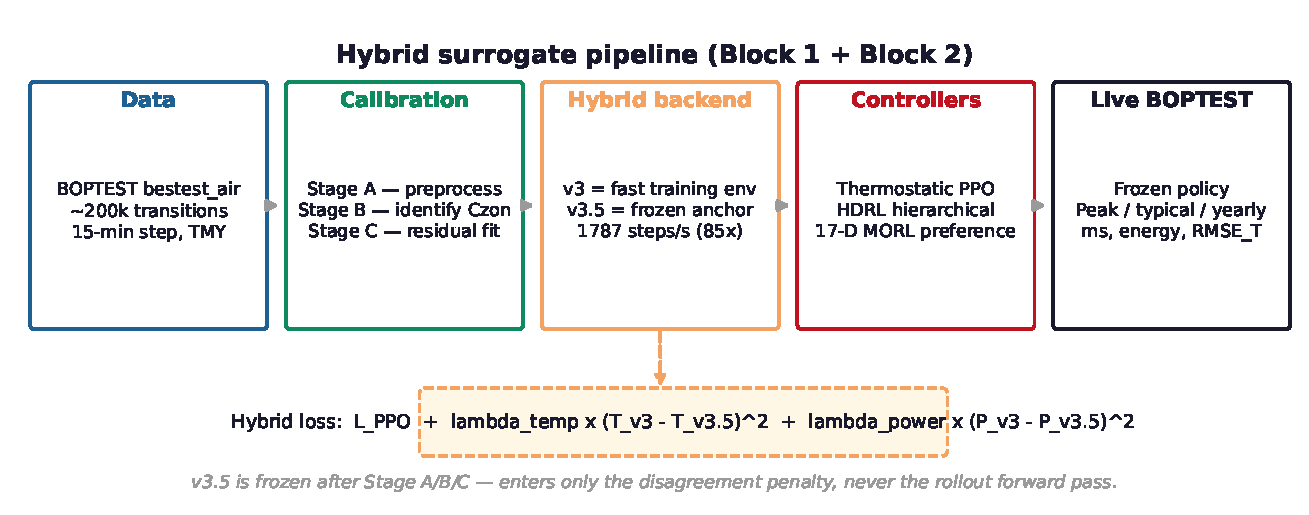
\includegraphics[width=0.95\linewidth]{figures/q1/C1_pipeline_overview.pdf}
  \caption{Information flow in the hybrid surrogate backend. The
  frozen physically informed model \texttt{v3.5} enters the policy
  training loss through the disagreement terms in
  Eq.~\eqref{eq:hybrid_loss} but not the policy's forward pass; the
  rollout environment is the smoother control-oriented surrogate
  \texttt{v3}.}
  \label{fig:pipeline}
\end{figure}
